\documentclass[11pt,letterpaper]{article}
\usepackage[utf8]{inputenc}
\usepackage[spanish,es-tabla,es-nodecimaldot]{babel} % Formato a español, Tabla en lugar de Cuadro
\usepackage{lmodern} % Fuente compatible
\usepackage{pgfplots} % Para poder realizar gráficas
    \pgfplotsset{compat=1.18}
\usepackage[T1]{fontenc}    % Permite utilizar otras tipografías
\usepackage{amsmath}
\usepackage[vmargin=2.5cm,hmargin=2cm]{geometry}
\usepackage{multicol}   % Unir columnas en tablas y formato a dos columnas
\usepackage{multirow}   % Unir filas en tablas
\usepackage{graphicx}   % Necesario para insertar gráficas
\usepackage{float}      % Corregir ubicación de imágenes y tablas
\usepackage{url}        % Hipervínculo a direcciones URL
\usepackage{listings}
%\usepackage{minted}    % Solo hace falta si se inserta código; requiere -shell-escape
\usepackage[none]{hyphenat} % Permite utilizar el comando \sloppy
\usepackage[small]{caption} % Reduce el tamaño de letra de los pies de figura y permite \captionof
\usepackage{hyperref}   % Agrega enlaces internos de las secciones, figuras y tablas.
\usepackage{color}      % Definición de colores
    \hypersetup{colorlinks=true, linkcolor=[rgb]{0,0,1}, citecolor=[rgb]{0,0,1}, urlcolor=[rgb]{0,0,1}}
\usepackage{xcolor}     % Permite definir un color para utilizarlo dentro del documento.
    \definecolor{gris}{RGB}{70,70,70}
    \definecolor{negro}{RGB}{40,40,40}
%%%%%%%% Modificación de los títulos de secciones %%%%%%%%%%
% Los nombres de las secciones van en MAYÚSCULAS y con letra más grande que el texto
\usepackage{titlesec}
\renewcommand\thesection{\Roman{section}}
\renewcommand\thesubsection{\Roman{subsection}}
\titlespacing*{\section}{0pt}{3mm}{1.5mm}
\titleformat{\section}[block]{\Large\bfseries\centering}{\thesection.}{0.6em}{\MakeUppercase}
\titleformat{\subsection}[block]{\normalsize\bfseries\raggedright}{\thesubsection.}{0.6em}{\MakeUppercase}
\usepackage{amssymb}
\pagestyle{plain} % Hojas enumeradas
%%%%%%%%%%%%%%%%%%%%%%%%%%%%%%%%%%%%%%%%%%%%%%%%%%%%%%%%%%%%%%%%%%%%%%%%%%%%%%

\newcommand{\colorhrule}[3]{\begingroup\color{#1}\rule{#2}{#3}\endgroup}
\setlength{\intextsep}{1mm}
\setlength{\columnsep}{5mm}

% -------------------------------------------------------------------
\begin{document}
\sloppy
\begin{center}
\begin{tabular}{cc}
\multirow{2}{3.5cm}{
\includegraphics[width=3cm]{udg_logo.jpeg}} & \huge{\textsc{\textbf{Universidad de Guadalajara}}}\\
 & \scriptsize{\textsc{CENTRO UNIVERSITARIO DE CIENCIAS EXACTAS E INGENIERÍAS}}\\[0.5mm]
 & \Large{\textsf{\textbf{Práctica 4. Superficie refractante}}}\\
 & \small{\textsf{Saul Emmanuel Ramirez Gonzalez [22382607]}}\\ \vspace{0.5mm}
 & \small{\textsf{Omar Emiliano Alcala Montes [220124466]}}\\ \vspace{0.5mm}
 & \small{\textsf{Luis Alberto Roman Verde [223826372]}}\\ \vspace{1mm}
 & \small{\textsc{Licenciatura en Física $|$ Óptica}}\\
 & \today\\
\end{tabular}
\end{center}

\begin{center}
\colorhrule{negro}{16.5cm}{1.2pt}
\end{center}
\begin{abstract}
\noindent En esta práctica se observó qué le pasa a un grupo de rayos de luz paralelos cuando atraviesan una pieza de acrílico de forma cilíndrica, es decir, cuando cruzan dos superficies refractantes curvas. Con una fuente de luz y una máscara de varias rendijas se obtuvieron siete rayos paralelos que se hicieron incidir sobre la cara curva del cilindro. Fue una práctica de observación, sin mediciones. Al salir del acrílico los rayos dejaron de ser paralelos y se juntaron en una zona muy cercana a la pieza, para luego volver a separarse. Se notó además que los rayos de las orillas se cruzaban antes que los del centro, de modo que no había un único punto de enfoque, y que en los bordes de los rayos aparecían colores. Estas observaciones coinciden con la ecuación de una superficie refractante esférica, que para un cilindro de acrílico predice un foco a una distancia de aproximadamente la mitad del radio detrás de la pieza, y con los fenómenos conocidos como aberración esférica y dispersión.

\end{abstract}
\begin{center}
\vspace{-0.1mm}
\colorhrule{gris}{16.5cm}{0.7pt}
\end{center}
\begin{multicols}{2}

\section{Introducción}
Una lupa, unos lentes de contacto o una gota de agua sobre una hoja tienen algo en común: todas son superficies curvas que doblan la luz.

En la práctica de la ley de Snell la luz cruzaba una frontera plana. Ahí todos los rayos que llegaban con el mismo ángulo se doblaban exactamente igual, y un grupo de rayos paralelos seguía siendo paralelo después de entrar al acrílico. Pero si la frontera es curva la historia cambia por completo, porque la normal ya no apunta en la misma dirección en todos los puntos de la superficie, y entonces cada rayo llega con un ángulo distinto, se dobla una cantidad distinta y, si la curva tiene la forma adecuada, todos terminan juntándose en una misma región.

Esa es, en el fondo, la idea de una lente.

En esta práctica hicimos pasar varios rayos paralelos a través de un cilindro de acrílico y observamos cómo se acercaban entre sí, dónde se cruzaban y qué tan bien lo hacían. No tomamos medidas; el objetivo fue mirar con cuidado y explicar lo que veíamos con la teoría.


\section{Objetivos}
El objetivo general fue observar cómo una superficie refractante curva cambia la dirección de un conjunto de rayos paralelos.

En particular queríamos ver si los rayos convergían después de atravesar el cilindro de acrílico, identificar en qué zona se juntaban y reconocer los defectos de enfoque que aparecen, para después comparar todo esto con lo que predice la ecuación de una superficie refractante esférica.


\section{Marco teórico}
Cada rayo que llega a una superficie, sea plana o curva, obedece la ley de Snell,
\begin{equation}
n_1 \sin\theta_1 = n_2 \sin\theta_2 ,
\label{eq:snell}
\end{equation}
donde los ángulos se miden desde la normal en el punto donde el rayo toca la superficie.

En una superficie curva la normal cambia de punto a punto. En un círculo es fácil saber hacia dónde apunta, porque siempre coincide con el radio, y de ahí sale todo lo demás.

\subsection{Ecuación de una superficie refractante esférica}
Supongamos que la frontera entre un medio de índice $n_1$ y otro de índice $n_2$ es un arco de círculo de radio $R$. Un objeto a una distancia $s_o$ de la superficie forma una imagen a una distancia $s_i$ del otro lado, y si los rayos están cerca del eje y llegan poco inclinados, a lo que se le llama aproximación paraxial, las dos distancias se relacionan con
\begin{equation}
\frac{n_1}{s_o} + \frac{n_2}{s_i} = \frac{n_2 - n_1}{R} .
\label{eq:superficie}
\end{equation}

Cuando los rayos llegan paralelos, como en esta práctica, es como si el objeto estuviera infinitamente lejos. El primer término desaparece y la distancia a la que se juntan los rayos, llamada distancia focal, queda
\begin{equation}
f = \frac{n_2 \, R}{n_2 - n_1} .
\label{eq:focal}
\end{equation}
Para luz que pasa del aire, con $n_1 = 1$, al acrílico, con $n_2 = 1.49$, esto da $f = 3.04 \, R$.

\subsection{Un cilindro completo}
Hay un problema con ese resultado. Si la pieza es un cilindro, su diámetro es $2R$, y como $3.04\,R$ es más que eso, los rayos llegan a la cara de salida antes de haberse juntado; ahí se encuentran con una segunda superficie curva, ahora del acrílico al aire, que los vuelve a doblar hacia el eje. Aplicando la ecuación \eqref{eq:superficie} dos veces se obtiene que el foco de un cilindro completo está, medido desde su centro, a
\begin{equation}
f = \frac{n \, R}{2 \, (n - 1)} ,
\label{eq:cilindro}
\end{equation}
lo que para el acrílico da $f = 1.52 \, R$. Restando el radio, la distancia del foco a la cara de salida del cilindro es
\begin{equation}
d = f - R = 0.52 \, R ,
\label{eq:distancia}
\end{equation}
es decir, los rayos deberían juntarse muy cerca de la pieza, a poco más de la mitad del radio.

\subsection{Aberración esférica}
La ecuación \eqref{eq:superficie} solo es exacta para rayos muy cercanos al eje. Los rayos que entran lejos del centro llegan a la superficie con ángulos grandes, y como el seno de la ley de Snell crece cada vez más despacio, estos rayos terminan doblándose de más y cruzan el eje antes que los centrales. El resultado es que no existe un punto de enfoque único, sino una zona alargada donde los rayos se van cruzando unos con otros. A este defecto se le llama aberración esférica, y la curva brillante que forman los rayos al cruzarse se conoce como cáustica.

\subsection{Dispersión}
Por último, el índice de refracción de un material cambia un poco con el color de la luz: es algo mayor para el azul que para el rojo. Por eso, cuando la fuente emite luz blanca, cada color se dobla de manera ligeramente distinta y en los bordes de los rayos aparecen franjas de colores.


\section{Material}
El equipo fue el mismo banco óptico de las prácticas anteriores:
\begin{itemize}
\item Fuente de luz incandescente.
\item Máscara con varias rendijas paralelas.
\item Pieza de acrílico de forma cilíndrica.
\item Hoja de papel blanco como superficie de observación.
\item Banco óptico.
\end{itemize}
Al igual que antes, el laboratorio se mantuvo a oscuras.


\section{Desarrollo experimental}
Colocamos la fuente de luz en un extremo del banco y frente a ella la máscara con rendijas, que dejaba pasar siete rayos delgados y paralelos. Sobre la mesa, delante de la máscara, extendimos una hoja blanca para poder ver la trayectoria de los rayos sobre el papel.

Después pusimos la pieza de acrílico.

La acomodamos sobre la hoja, de pie sobre una de sus caras planas, de manera que los siete rayos golpearan su costado curvo y el rayo del centro pasara justo por la mitad del cilindro. Con las luces apagadas, observamos cómo entraban los rayos, cómo salían por el otro lado y en qué zona se cruzaban, y movimos ligeramente la pieza a un lado y a otro para ver si el patrón cambiaba. La figura \ref{fig:frente} muestra el arreglo visto desde la fuente.

\begin{center}
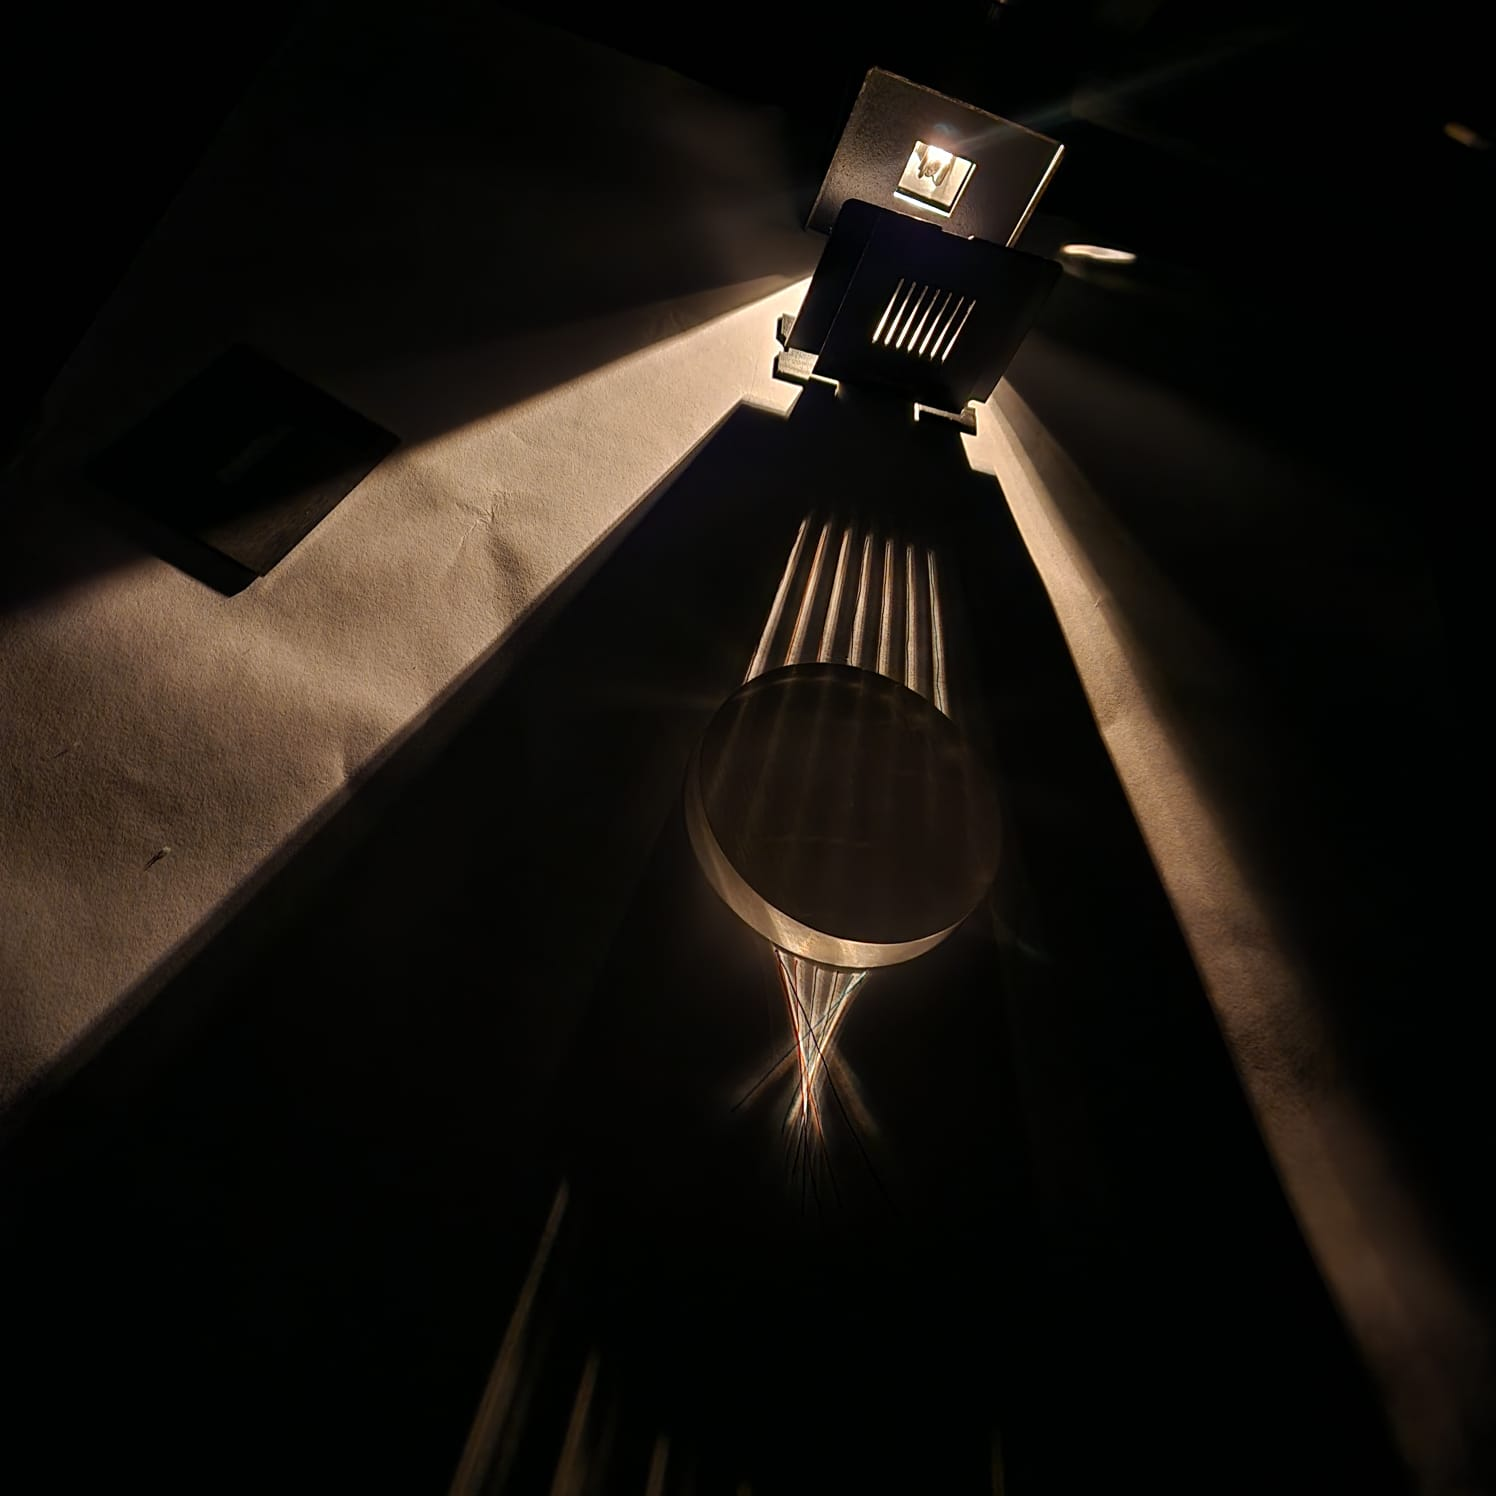
\includegraphics[width=\columnwidth]{rayos_frente.jpg}
\captionof{figure}{Arreglo experimental. Los siete rayos paralelos salen de la máscara, atraviesan el cilindro de acrílico y se cruzan detrás de él.}
\label{fig:frente}
\end{center}

Como no se tomaron medidas, todo lo que sigue se basa en la observación directa y en las fotografías.


\section{Resultados}
Lo primero que se vio fue que, antes de llegar al acrílico, los siete rayos avanzaban paralelos y con la misma separación entre ellos, tal como salían de la máscara.

Al otro lado, todo cambió.

Los rayos salieron del cilindro inclinados hacia el centro y se juntaron muy cerca de la pieza, a una distancia bastante menor que su radio, para después cruzarse y abrirse de nuevo en forma de abanico. Así se aprecia en la figura \ref{fig:lado}, tomada desde un costado.

\begin{center}
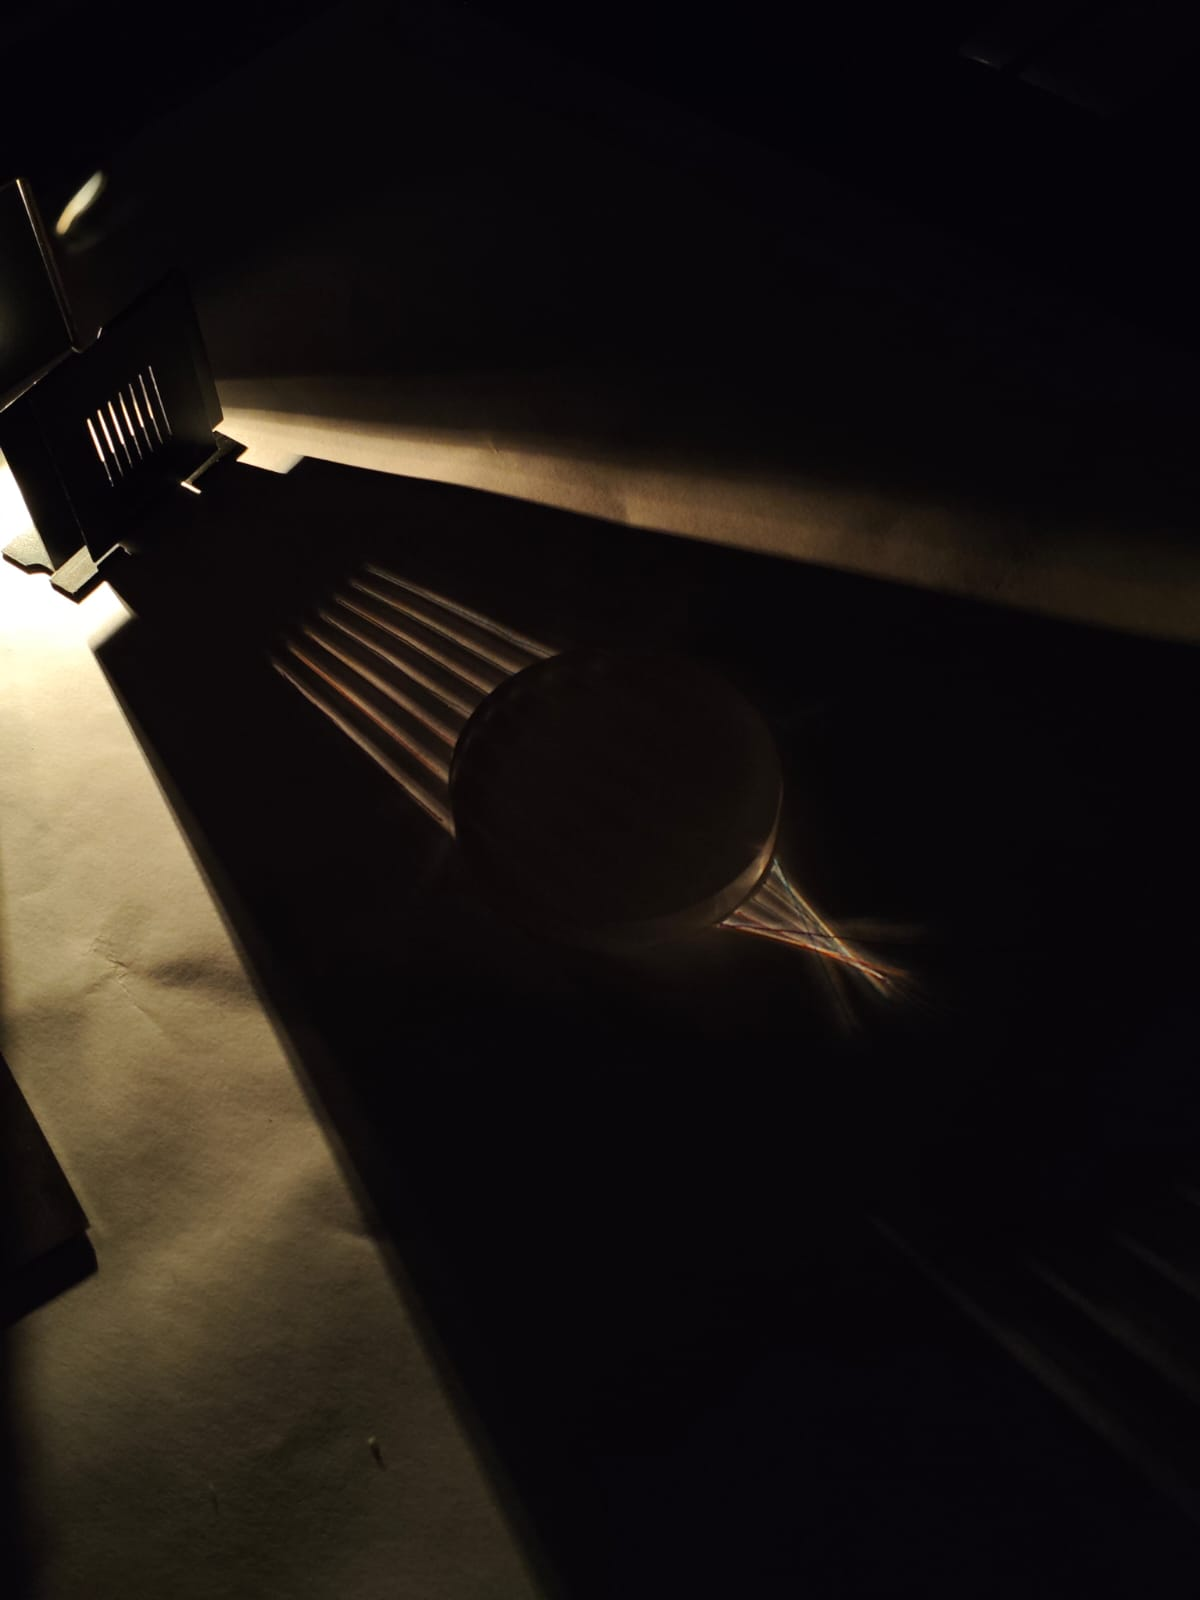
\includegraphics[width=0.8\columnwidth]{rayos_lado.jpg}
\captionof{figure}{Vista lateral. Los rayos paralelos entran por la izquierda y, al salir del cilindro, convergen y se cruzan a poca distancia de su cara de salida.}
\label{fig:lado}
\end{center}

Mirando con más atención, se notó que los rayos no se juntaban todos en un mismo punto. Los dos de las orillas se cruzaban primero, prácticamente pegados al acrílico, los siguientes un poco más adelante, y el rayo central atravesaba la pieza sin desviarse y era el último en ser alcanzado por los demás. En lugar de un punto brillante se formaba una pequeña región alargada, con forma de punta de flecha, donde las líneas se iban cruzando unas con otras.

Por último, en esa zona de cruce los rayos ya no se veían blancos. Sus bordes mostraban colores, rojizos de un lado y azulados del otro, algo que antes de entrar al acrílico no ocurría.

Para comparar con la teoría, la ecuación \eqref{eq:distancia} indica que en un cilindro de acrílico los rayos cercanos al eje deberían juntarse a $0.52\,R$ de la cara de salida. Esto coincide con lo observado: el cruce ocurrió a una distancia de aproximadamente la mitad del radio de la pieza, y no a más de tres radios, como habría pasado con una sola superficie curva según la ecuación \eqref{eq:focal}.


\section{Análisis y conclusiones}
Lo que más llama la atención es lo rápido que se enfocan los rayos. Con una sola superficie curva de acrílico el foco estaría a más de tres radios, pero en el cilindro los rayos se cruzaron prácticamente pegados a la pieza, y la razón es que cruzan dos superficies curvas y no una: la de entrada empieza a juntarlos, la de salida los vuelve a doblar en la misma dirección y, sumando el efecto de las dos, el foco queda a $1.52\,R$ del centro, como indica la ecuación \eqref{eq:cilindro}.

En otras palabras, el cilindro se comporta como una lente convergente muy potente.

El segundo resultado es la aberración esférica. Que los rayos de las orillas se crucen antes que los del centro es exactamente lo que se espera, porque llegan a la superficie con ángulos de incidencia grandes, donde la aproximación paraxial ya no funciona y la ecuación \eqref{eq:snell} los dobla más de lo que predice la ecuación \eqref{eq:superficie}. En el cilindro este efecto es muy notorio porque los rayos de los extremos entran lejos del eje en comparación con el radio de la pieza. Por eso las lentes de calidad no usan superficies tan curvas, o combinan varias lentes para corregirlo, y por eso también las cámaras dan imágenes más nítidas cuando se cierra el diafragma y solo pasan los rayos centrales.

Los colores tienen otra explicación. El acrílico no dobla igual todos los colores, y como la fuente da luz blanca, cada componente se enfoca en un lugar un poquito distinto. Este defecto se llama aberración cromática.

Hay que reconocer que, al no haber mediciones, la comparación con la teoría es solo cualitativa. Habría sido útil medir el radio de la pieza y la distancia del cruce de los rayos centrales hasta la cara de salida para comprobar el valor de $0.52\,R$, así como la distancia de cruce de los rayos de las orillas para tener una idea de qué tan grande es la aberración.

En conclusión, una superficie curva de acrílico hace converger un haz de rayos paralelos, y un cilindro completo, al tener dos superficies, lo enfoca a muy poca distancia de su cara de salida, en acuerdo con la ecuación de una superficie refractante esférica aplicada dos veces. Además se observaron con claridad dos limitaciones de las lentes reales: la aberración esférica, por la que los rayos de las orillas se enfocan antes que los centrales, y la aberración cromática, por la que cada color se enfoca en un punto diferente.




\section{Bibliografía}
Las fuentes consultadas para preparar este reporte fueron las siguientes.

\begin{enumerate}
\item Hecht, E. (2017). \textit{Optics} (5a ed.). Pearson.
\item Serway, R. A. y Jewett, J. W. (2019). \textit{Física para ciencias e ingeniería}, volumen 2 (10a ed.). Cengage Learning.
\item Feynman, R. P., Leighton, R. B. y Sands, M. (2010). \textit{The Feynman Lectures on Physics}, volumen I, capítulo 26: Optics, the principle of least time. California Institute of Technology. Recuperado de \url{https://www.feynmanlectures.caltech.edu/I_26.html}
\end{enumerate}


\end{multicols}

\end{document}
